\begin{figure}[htbp]
\centering
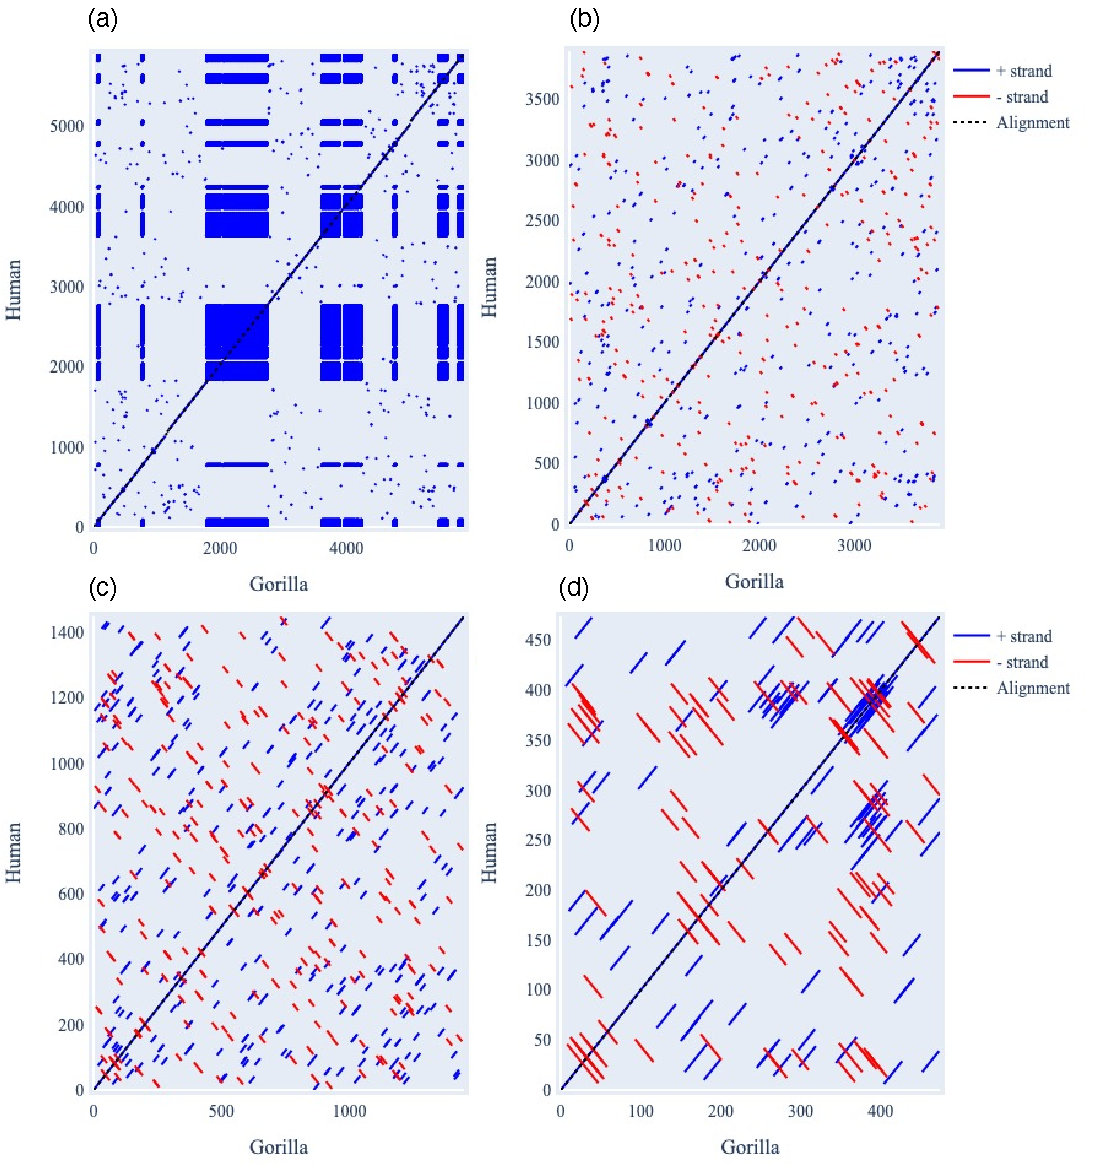
\includegraphics[width=\textwidth]{figures/diagrams/primate_dotplots.pdf}
\caption{\textbf{Dotplots of an intronic and CDS alignment before and after filtering}. \textbf{(a)}, intronic pre-filtering, \textbf{(b)} intronic post-filtering, \textbf{(c)} CDS pre-filtering, \textbf{(d)}, CDS post-filtering. Each point on the plot indicates where the nucleotide is identical between the two sequences. Long stretches of identity between the sequences form a diagonal. Long stretches of tandem repeats show up as large blocks of colour, visible in (a). The window was 20bp long, a match was considered if $>13$bp of the window of 20 were identical between the sequences. }
\label{fig:dotplots}
\end{figure}